\documentclass[journal]{IEEEtran}

\usepackage[T1]{fontenc}
\usepackage[utf8]{inputenc}
\usepackage{cite}
\usepackage{amsmath,amssymb,amsfonts}
\usepackage{graphicx}
\usepackage{xcolor}
\usepackage{booktabs}
\usepackage[hidelinks]{hyperref}

\newcommand{\mbf}[1]{\mathbf{#1}}
\newcommand{\bs}[1]{\boldsymbol{#1}}
\newcommand{\todo}[1]{\textcolor{red}{[#1]}}

\graphicspath{{../makale2_revizyon/}}
\emergencystretch=1em
\begin{document}
\renewcommand{\abstractname}{Özet}
\renewcommand{\IEEEkeywordsname}{Anahtar Kelimeler}
\renewcommand{\figurename}{Şekil}
\renewcommand{\tablename}{Tablo}
\renewcommand{\refname}{Kaynaklar}

\title{Hareketli Kullanıcılara Hizmet Eden Yeniden Yapılandırılabilir Akıllı Yüzeyler için Gecikme Farkındalıklı Faz Optimizasyonu}

\author{Seda~Savaşçı~Şen, Ali~Çalhan ve Murtaza~Cicioğlu%
\thanks{(Sorumlu yazar: Seda Savaşçı Şen.) Bu belge, IEEE Transactions on Wireless Communications'a gönderilen İngilizce makalenin birebir Türkçe çalışma çevirisidir; şekillerdeki etiketler İngilizce bırakılmıştır.}%
\thanks{S.~Savaşçı~Şen, Düzce Üniversitesi Elektrik-Elektronik Mühendisliği Bölümü, Düzce, Türkiye (e-posta: sedasavascisen@duzce.edu.tr).}%
\thanks{A.~Çalhan, Düzce Üniversitesi Bilgisayar Mühendisliği Bölümü, Düzce, Türkiye (e-posta: alicalhan@gmail.com).}%
\thanks{M.~Cicioğlu, Bursa Uludağ Üniversitesi Bilgisayar Mühendisliği Bölümü, Bursa, Türkiye (e-posta: murtazacicioglu@uludag.edu.tr).}}

\markboth{IEEE Transactions on Wireless Communications}%
{Hareketli Kullanıcılar için Gecikme Farkındalıklı RIS Faz Optimizasyonu}

\maketitle

\begin{abstract}
Yürüyen bir kullanıcı kanalı onlarca milisaniye içinde değiştirir; buna karşın yeniden yapılandırılabilir akıllı yüzey (RIS) faz optimizasyon yöntemleri genellikle kendilerine verilen kanalda ulaştıkları hızla karşılaştırılır. Biz bunun yerine her yöntemi, işini bitirdiği anda var olan kanalda, yani \emph{etkin hızı} ile ve ölçülmüş gecikmelerle değerlendiriyoruz; kurgu, 32 elemanlı bir RIS'e sahip iç mekân ofis ortamında dar bantlı, çok kullanıcılı, çok girişli tek çıkışlı bir aşağı bağlantıdır. Birincisi, başlangıç kanalında yüksek hıza ulaşan iki çözücü, koordinat inişi ve uzun koşulu Adam, 0.9--5.9~s gerektirir ve 2.5~ms süren tek kullanıcılı bir sezgisel yönteme kaybeder. İkincisi, daha fazla yineleme yalnızca bir noktaya kadar yarar sağlar: 1.5~m/s'de Adam'ın etkin hızı 4--6 adımda tepe yapar ve onu 48 adıma kadar koşturmak \%14 kaybettirir; 10~km/h'de tepe 3 adımdadır. Optimumu, bir küçük gecikme modelinin açıkladığı gibi, adım süresinin Doppler frekansına göre büyüklüğü belirler. Üçüncüsü, eşit adımda ayarlanmış Adam'ı geçen öğrenilen bir güncelleme kuralı, gecikme tek iş parçacığında ölçüldüğünde daha hızlı Adam yapılandırmaları tarafından baskınlanır. Taze bir ön kodlayıcının pilotlarını hesaba katmak hızları düşürür, ancak yavaş çözücüler ayarlanmış Adam'ın gerisinde kalır. Ölçülen adım maliyetinde yaya kullanıcılar için hangi yöntemin en iyi olduğuna yakınsama değil, gecikme karar verir.
\end{abstract}

\begin{IEEEkeywords}
Yeniden yapılandırılabilir akıllı yüzey, faz optimizasyonu, hareketlilik, kanal eskimesi, hesaplama gecikmesi.
\end{IEEEkeywords}

\section{Giriş}
\label{sec:intro}

\IEEEPARstart{Y}{eniden} yapılandırılabilir akıllı yüzey (RIS), bir binanın engellenmiş bir köşesini kapsama altındaki bir köşeye dönüştürebilir~\cite{Basar2019Access,DiRenzo2020JSAC,Wu2021TCOM}; 256 elemanlı bir RIS verici anten olarak görev yapmıştır~\cite{Dai2020Access} ve bir başka prototip, bir beton duvarın içinden geçen bir bağlantıyı güçlendirmiştir~\cite{Pei2021TCOM}. Ancak bir yüzey, yalnızca pasif elemanları sinyali kullanıcının \emph{şu an} bulunduğu yere yönlendirdiğinde yardımcı olur; kullanıcının \emph{önceden} bulunduğu yere değil. Bu fazları seçmek, yinelemeli çözücülerle~\cite{Wu2019TWC,Abeywickrama2020TCOM,Pan2020TWC,Guo2020TWC,Choi2024TCOM} ve giderek artan ölçüde öğrenilmiş politikalarla~\cite{Huang2020JSAC} ele alınan, zor ve dışbükey olmayan bir problemdir. Bu yöntemler genellikle kendilerine verilen kanal üzerinde ulaştıkları hızla karşılaştırılır.

Bu karşılaştırma bir yarışı gizler. Bir ofiste yürüyen bir kişi radyo kanalını onlarca milisaniye içinde değiştirir; özenli bir çözücü ise saniyeler gerektirebilir. En iyi yanıt hazır olduğunda soru değişmiş olur. Bu durumda zamanında teslim edilen kaba bir faz, geç teslim edilen mükemmel bir fazı geçebilir ve daha fazla yineleme koşturmak sonucu daha iyi değil, daha kötü yapabilir.

Bu makale bu yarışı ölçer. Her yöntemi, işini bitirdiği anda var olan kanal üzerinde, yani \emph{etkin hızı} ile; gecikmeleri bir CPU üzerinde ölçerek, yürüyen kullanıcıların bulunduğu bir iç mekân ofisinde ve 3GPP TR~38.901 kanal modeliyle~\cite{3gpp_channel} değerlendiriyoruz. Soru, bir baz istasyonunun (BS) karşılaştığı sorudur: zaman hesaba katıldığında hangi yöntemi koşturmalı ve ne kadar süreyle? Bu çalışma, sinüs--kosinüs gösterimine dayanan tek geçişli faz öngörücümüzü~\cite{SavasciSen2026AISY}, koşma süresi maliyet olarak yansıtıldığında böyle bir hızın ne zaman karşılığını verdiğini sorarak sürdürmektedir.

\subsection{Katkılar}
\begin{enumerate}
    \item \textbf{Gecikmeyi hesaba katan bir ölçüt.} Etkin hızı tanımlıyor (Bölüm~\ref{sec:framework}) ve bu ölçüt altında, kâğıt üzerinde en iyi hıza sahip çözücülerin, yaya kullanıcılar için ve ölçülen adım maliyetinde, milisaniyeler süren tek kullanıcılı bir sezgisel yönteme yenildiğini gösteriyoruz.
    \item \textbf{Optimal bir yineleme sayısı.} Daha fazla yineleme yalnızca bir noktaya kadar yardımcı olur. En iyi adım sayısı tek bir nicelikle, yani Doppler frekansına göreli adım süresiyle belirlenir ve bir küçük gecikme modeli bunun nasıl ölçeklendiğini açıklar. Dar bant modelde optimum, ikinci bir klasik optimize edici, daha büyük bir yüzey ve standartlaştırılmış her iç mekân hızı için de varlığını korur.
    \item \textbf{Periyodik işletim.} BS sürekli olarak yeniden optimize ettiğinde, ne sıklıkla güncelleme yapılacağına pilot ek yükü karar verir ve kısa güncellemeler (en fazla 8 adım) yeterlidir.
    \item \textbf{Saat karşısında öğrenme.} Ayarlanmış bir klasik optimize ediciyi adım başına yenen bir öğrenilen güncelleme kuralı, milisaniye başına ona yenilir.
    \item \textbf{Ana varsayımın bedeli.} Ana sonuçlar, BS'nin ön kodlayıcısını güncel kanaldan yenilediğini varsayar; sonuçların buna ne kadar bağlı olduğunu nicelendiriyor, ayrıca pilot yayın süresini, kestirim hatasını ve ayrık fazları ekliyoruz.
\end{enumerate}

\section{İlgili Çalışmalar}
\label{sec:related_work}

\emph{RIS faz optimizasyonu.} Ortak ön kodlama ve faz tasarımı; dönüşümlü optimizasyon ve yarı tanımlı gevşetme~\cite{Wu2019TWC}, faza bağımlı pratik genlik modelleri~\cite{Abeywickrama2020TCOM}, blok koordinat inişi~\cite{Pan2020TWC}, kesirli programlama~\cite{Guo2020TWC}, sabit nokta ve manifold yöntemleri~\cite{Yu2019ICCC} ve~\cite{Shi2011TSP} çalışmasındaki algoritmanın üzerine kurulan ağırlıklı en küçük ortalama karesel hata (WMMSE) yöntemleri~\cite{Choi2024TCOM} ile ele alınmıştır. Bu çalışmalar ulaşılan amaç fonksiyonu değerini raporlar; koşma süresi genellikle bir karmaşıklık mertebesi olarak verilir ve ölçüldüğü durumlarda da sabit kanal gerçekleşmeleri üzerinde ölçülür~\cite{Abeywickrama2020TCOM,Yu2019ICCC,Shi2011TSP,Cao2022TWC}; eş evrelilik süresiyle karşılaştırılmaz.

\emph{Öğrenme.} Öğrenilmiş politikalar arasında ortak ön kodlama ve faz tasarımı için derin pekiştirmeli öğrenme~\cite{Huang2020JSAC} ve yansıtmayı doğrudan pilotlardan öğrenme~\cite{Jiang2021JSAC} yer alır. Algoritma açma (unrolling), bir optimize edicinin yinelemelerini ağ katmanlarına dönüştürür~\cite{Monga2021SPM}; bu yaklaşım RIS hüzme oluşturmaya~\cite{Liu2022TWC}, MIMO sezimine~\cite{Samuel2019TSP} ve WMMSE ön kodlamaya~\cite{Hu2021TWC,Pellaco2022OJCOMS} uygulanmıştır ve eğitilmiş ağlar WMMSE'yi onun koşma süresinin küçük bir kesrinde yaklaşık olarak gerçekleyebilir~\cite{Sun2018TSP}. Her fazın sinüs ve kosinüsünü öngörmek, doğrudan faz regresyonunun $\pm\pi$ süreksizliğini ortadan kaldırır~\cite{SavasciSen2026AISY}. Öğrenilen yöntemler genellikle hızla gerekçelendirilir, ancak bu hız nadiren kanalın ne kadar hızlı değiştiğiyle ilişkilendirilir; her ikisi tek bir makinede zamanlandığında bile~\cite{Samuel2019TSP,Sun2018TSP,Hu2021TWC,Liu2022TWC}, klasik taban çizgisi aynı gecikmeye kadar değil, yakınsamaya ya da sabit bir yineleme sayısına kadar koşturulur.

\emph{Hareketlilik ve güncelliğini yitirmiş kanallar.} İki aşamalı kestirim kullanan, araca monte edilmiş kırıcı bir yüzey, hızlı sönümlemeyi yavaş sönümlemeye dönüştürür~\cite{Huang2022TWC}. RIS için kanal eskimesi~\cite{Papazafeiropoulos2023TVT} ve güncelliğini yitirmiş kanal bilgisi~\cite{Zhang2022TCOM} analiz edilmiştir; öngörücü hüzme oluşturma, hüzmeleri hızlı insansız hava araçlarının öngörülen konumlarına yöneltir~\cite{Liu2021WCL} ve etkin algılama hareketli kullanıcıları izler~\cite{Han2025TWC}. Eskime, büyük MIMO'da klasik bir konudur~\cite{Truong2013JCN,Chopra2018TWC}; yayın kanallarında sınırlı kanal geri beslemesi de öyledir~\cite{Jindal2006IT}. İki zaman ölçekli tasarımlar fazları kanal istatistiklerinden, ön kodlayıcıyı ise anlık kanallardan günceller~\cite{Zhao2021TWC,Cao2022TWC}. Pratik yüzeylerin birkaç bitlik faz çözünürlüğü vardır~\cite{Wu2020TCOM,Zhao2024OJCOMS}; Bölüm~\ref{sec:res_robust}, sürekli faz sonuçlarımıza 1--3 bitlik fazları ekler. Bu çalışmalarda kanal edinimi ile kullanımı arasındaki gecikme, modellendiği yerde sabittir; hesaplama bir neden olarak anıldığı yerde bile~\cite{Truong2013JCN} böyledir; optimize edicinin kendi koşma süresi en fazla bir uygulanabilirlik kontrolü ya da sabit bir ek yüktür~\cite{Ryu2026arXiv,Liu2021WCL} ve eskimeye dahil edilmez.

\emph{Boşluk.} Bildiğimiz kadarıyla hiçbir RIS çalışması her yöntemi kendi ölçülmüş tamamlanma anındaki kanal üzerinde değerlendirmemekte, bunun optimal bir yineleme sayısı ortaya çıkardığını göstermemekte ya da öğrenilen ve klasik optimize edicileri hem eşit adımda hem de eşit ölçülmüş sürede karşılaştırmamaktadır.

\section{Sistem ve Kanal Modeli}
\label{sec:system}

\subsection{Sinyal Modeli}
Yarım dalga boyu aralıklı $N_t=8$ antenden oluşan düzgün doğrusal diziye sahip bir baz istasyonu (BS), $K=4$ tek antenli kullanıcıya doğrudan bir bağlantı ve $N=32$ pasif elemanlı bir RIS ($8\times 4$ düzlemsel dizi) üzerinden hizmet verir; Bölüm~\ref{sec:res_scaling} ayrıca $N=64$ durumunu da kullanır. Fazlar $\bs{\theta}\in[0,2\pi)^N$, $\mbf{v}=e^{j\bs{\theta}}$ ve ön kodlayıcı $\mbf{W}=[\mbf{w}_1,\dots,\mbf{w}_K]$ olmak üzere, $k$ kullanıcısı şu sinyali alır:
\begin{equation}
    y_k = \left(\mbf{h}_{d,k}^H + \mbf{g}_k^H \operatorname{diag}(\mbf{v})\mbf{F}\right)\sum_{j=1}^K \mbf{w}_j s_j + n_k ,
    \label{eq:signal}
\end{equation}
burada $\mbf{F}\in\mathbb{C}^{N\times N_t}$ BS--RIS kanalı, $\mbf{g}_k^H$ RIS--kullanıcı kanalı, $\mbf{h}_{d,k}^H$ doğrudan kanaldır ve gürültü $n_k\sim\mathcal{CN}(0,\sigma^2)$ biçimindedir. Parantez içindeki etkin kanal $\mbf{h}_k^H(\bs{\theta})$ ile gösterildiğinde, $k$ kullanıcısının hızı $R_k=\log_2(1+\mathrm{SINR}_k)$ olur; burada sinyal-girişim-artı-gürültü oranı $\mathrm{SINR}_k = |\mbf{h}_k^H \mbf{w}_k|^2/(\sum_{j\ne k}|\mbf{h}_k^H \mbf{w}_j|^2 + \sigma^2)$ biçimindedir. Ön kodlayıcı, etkin kanal üzerinde düzenlileştirilmiş sıfır zorlamadır (ZF)~\cite{Peel2005TCOM}; düzenlileştirici $\lambda = K\sigma^2/P$ ve toplam güç $P$ olarak alınır. Amaç fonksiyonu en düşük kullanıcı hızıdır; bu, RIS destekli çok girişli tek çıkışlı (MISO) sistemler için~\cite{Nadeem2020TWC} çalışmasında da kullanılan bir adalet ölçütüdür:
\begin{equation}
    \max_{\bs{\theta}} \; \min_k R_k(\bs{\theta}),
    \label{eq:maxmin}
\end{equation}
Adam, Armijo ve öğrenilen güncelleme (Bölüm~\ref{sec:method}) bu problemi pürüzsüz vekil $-\tfrac{1}{\beta}\log\sum_k e^{-\beta R_k}$, $\beta=8$ üzerinden optimize eder; koordinat inişi ve uzun koşulu Adam referansı ise katı minimumu maksimize eder.

\subsection{Geometri ve Yayılım}
\begin{figure*}[t]
\centering
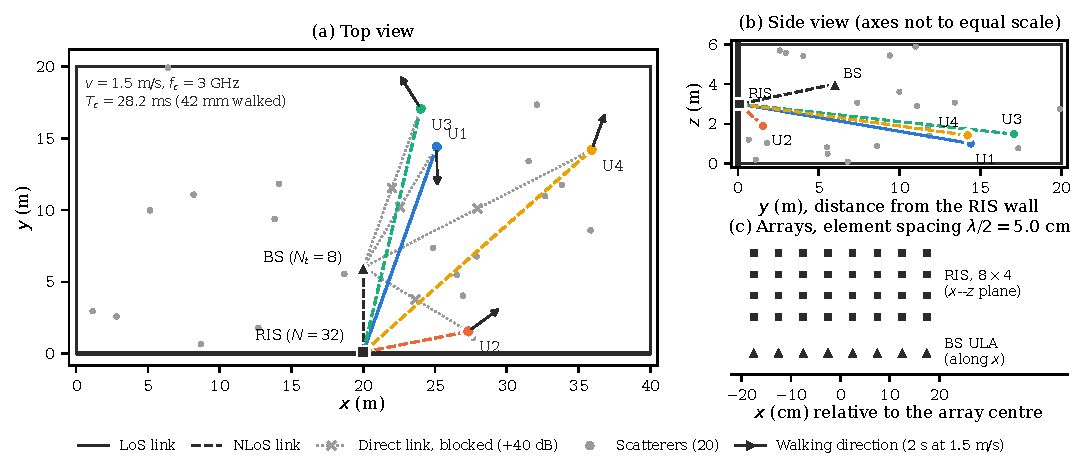
\includegraphics[width=\textwidth]{figures/fig_scenario.pdf}
\caption{Benzetimi yapılan senaryo (eskime kümesinin ilk senaryosu). (a)~$40\times20\times6$~m boyutlu ofisin üstten görünümü: BS $(20,6,4)$~m konumunda, duvara monte edilmiş RIS $(20,0.1,3)$~m merkezli, 1.5~m/s hızla yürüyen dört kullanıcı, 20 noktasal saçıcı. Çizgi stili: her bağlantının görüş hattı (LoS) durumu. Bütün doğrudan bağlantılar 40~dB'lik engellemeyi taşır. Oklar: 2~s'lik yürüyüş; bir eş evrelilik süresi içinde bir kullanıcı yalnızca 42~mm yer değiştirir. (b)~Yandan görünüm. (c)~Eleman yerleşimleri.}
\label{fig:scenario}
\end{figure*}
Oda $40\times 20\times 6$~m boyutundadır (Şekil~\ref{fig:scenario}). RIS bir duvar üzerinde $(20, 0.1, 3)$~m noktasında merkezlenmiştir; BS ise $(20, 6, 4)$~m noktasında, panelin bakış ekseni (boresight) üzerinde ve panelin Fraunhofer uzaklığının ötesindedir. Kullanıcılar 1--2~m yüksekliklere düzgün dağılımla yerleştirilir. Taşıyıcı frekansı $f_c=3$~GHz, bant genişliği 20~MHz, iletim gücü 20~dBm, BS anten kazancı 5~dBi ve gürültü faktörü 7~dB'dir. Bütün bağlantılar 3GPP TR~38.901 iç mekân ofis modelini~\cite{3gpp_channel} izler: bu modelin yol kaybı, karma ofis LoS olasılığı, Rician faktörü ve 5~m'de üstel uzamsal korelasyonlu log-normal gölgelemesi (TR~38.901, LoS için 10~m, görüş hattı dışı (NLoS) için 6~m öngörür). NLoS bileşenleri, bir senaryonun bütün bağlantılarınca paylaşılan noktasal saçıcılardan gelir. Kademeli (cascaded) genlik, $\cos^q$ güç örüntülü ($q{=}1$) serbest uzay iki atlamalı modeli~\cite{Tang2021TWC} izler; her atlamaya TR~38.901 ek kaybını ve gölgelemesini ekliyoruz. Bizim eleman kazancımız $2(2q{+}1)$, Tang'in $2(q{+}1)$ kazancını aşar; ikincisi mutlak hızları yaklaşık \%5 düşürür ve $L^\star$ ile en iyi yöntemi değiştirmez. RIS, doğrudan yolun engellendiği yerlere konuşlandırıldığı için doğrudan bağlantı fazladan 40~dB kayıp taşır.

\subsection{Hareketlilik}
Kullanıcılar $v=1.5$~m/s (5.4~km/h) hızla düz çizgiler boyunca yürür ve duvarlardan yansır. Bu değer, 3GPP iç mekân sıcak nokta değerlendirmesindeki 3~km/h~\cite{3gpp_tr38913} ile iç mekân hareketliliğinin değerlendirildiği IMT-2020 yaya sınıfının 10~km/h üst sınırı~\cite{itu_m2410} arasında yer alır; Bölüm~\ref{sec:res_sensitivity} ana ölçümleri bu hızlarda ve daha yüksek hızlarda tekrarlar. Saçıcılar, yol kazançları, LoS durumları, gölgeleme ve $\mbf{F}$ sabit tutulur; yalnızca kullanıcılar hareket eder ve $\mbf{g}_k(t)$ ile $\mbf{h}_{d,k}(t)$ her anda geometriden yeniden hesaplanır. Referans zaman ölçeği Doppler frekansı $f_d=vf_c/c=15$~Hz'dir; buna karşılık gelen eş evrelilik süresi $T_c=\sqrt{9/(16\pi)}/f_d\approx0.423/f_d=28.2$~ms'dir.

\emph{Sınırlamalar.} Sabit saçıcılar, kanalın saniyeler mertebesinde gerçek bir kanaldan daha az değişmesine yol açar; bu nedenle 200~ms ötesindeki etkin hızlar yavaş yöntemler için iyimserdir; gerçek değerler bunlar ile Tablo~\ref{tab:aging} içindeki bayat taban arasında olmalıdır. Saçılmış yol kazançları her BS anteni için bağımsız olarak çekilir; bu da bütün mutlak hızları iyimser kılar; Bölüm~\ref{sec:res_sensitivity} ana ölçümleri paylaşılan kazançlarla tekrarlar. Ana sonuçlarda kanal bilgisi, eklediğimiz kanal edinme gecikmesi dışında kusursuzdur; Bölüm~\ref{sec:res_robust} kestirim hatası ekler. Model dar banttır (hüzme kayması yoktur) ve $N=32$ için uzak alandadır; $N=64$ için BS (6.0~m uzaklıkta) 6.4~m'lik Fraunhofer uzaklığının hemen içinde kalır ve kanal, eleman başına tam uzaklıkları kullanır.

\section{Gecikmeye Duyarlı Değerlendirme Çerçevesi}
\label{sec:framework}

\subsection{Etkin Hız}
Bir $A$ yöntemi $\mathcal{H}(0)=\{\mbf{F},\mbf{g}_k(0),\mbf{h}_{d,k}(0)\}$ kanalını alsın, $\bs{\theta}_A$ fazını döndürsün ve bunu yapmak için $\tau_A$ duvar saati süresine ihtiyaç duysun.

\textbf{Tanım 1 (Etkin hız).} $A$ yönteminin etkin hızı, yöntem işini bitirdiğinde mevcut olan kanal üzerindeki en düşük kullanıcı hızıdır,
\begin{equation}
    R^{\mathrm{eff}}_A = \min_k R_k\big(\bs{\theta}_A;\,\mathcal{H}(\tau_A)\big),
    \label{eq:effective_rate}
\end{equation}
burada ön kodlayıcı $\mathcal{H}(\tau_A)$ kanalından yeniden hesaplanır.

Ön kodlayıcı, BS'nin taze pilotlara sahip olduğu her durumda yinelediği kapalı biçimli bir hesaplamadır; RIS fazı ise gecikmesini ölçtüğümüz yinelemeli optimizasyonu gerektirir. Bu nedenle Tanım~1 fazın eskimesine izin verir ve hüzmeyi taze tutar; bu ayrım, iki zaman ölçekli tasarımlardakine~\cite{Zhao2021TWC} benzer. Bölüm~\ref{sec:res_beam} ve~\ref{sec:res_robust} bu varsayımın bedelini ölçer.

\subsection{Neden Optimal Bir Adım Sayısı Vardır}
$L$ adım boyunca koşturulan yinelemeli bir yöntem için $t=0$ anındaki en düşük hızını $r_0(L)$, gecikmesini $\tau(L)$ ve kendi çalışma süresi boyunca eskime nedeniyle kaybedilen hızı $\Delta(L)=r_0(L)-\min_k R_k(\bs{\theta}_L;\mathcal{H}(\tau(L)))$ ile gösterelim; böylece $R^{\mathrm{eff}}(L)=r_0(L)-\Delta(L)$ olur. Her adım $r_0$ değerini azalan getiriyle artırırken $\Delta$, $\tau$ ile birlikte büyür. Bir adım ancak şu koşul sağlandığı sürece karşılığını verir:
\begin{equation}
    r_0(L+1)-r_0(L) \;>\; \Delta(L+1)-\Delta(L),
    \label{eq:marginal}
\end{equation}
ve etkin hız bu koşulun sağlanmadığı noktada tepe yapar: \emph{içsel optimum} $L^\star$. Bu optimum; optimize ediciye, onun adım başına gecikmesine ve kanal değişiminin hızına birlikte bağlıdır. $R^{\mathrm{eff}}$ fonksiyonunun tek tepeli olup olmadığı deneysel bir sorudur (Bölüm~\ref{sec:res_optimum}).

\subsection{Eşit Adıma Karşı Eşit Milisaniye}
Öğrenilen bir adım $c$ klasik adım kadar zaman alıyorsa, eşit adımlı bir karşılaştırma öğrenilen yönteme $c$ kat zaman bütçesi verir. Bu nedenle ölçülen eşit süre altında da karşılaştırma yapıyoruz.

\textbf{Tanım 2 (Baskınlık).} $\tau_B\le\tau_A$ ve $r_{0,B}\ge r_{0,A}$ ise ve eşitsizliklerden biri kesinse, $B$ yapılandırması $A$ yapılandırmasını baskınlar.

Baskınlanmış bir yapılandırma, hiçbir gecikme bütçesinde daha iyi seçenek değildir.

\subsection{Normalize Adım Maliyeti ve Küçük Gecikme Modeli}
Kanal değişimi, kullanıcının dalga boyu cinsinden kat ettiği uzaklığa ($f_d\tau$) bağlıdır. Bir optimize edici adım başına $\Delta T$ süre harcıyorsa, $L$ adım sonraki gecikmesi bu birimlerde $Lx$ olur; burada
\begin{equation}
    x = \Delta T\, f_d .
    \label{eq:x}
\end{equation}
Modelimizde $\Delta T$ değerini ölçeklemek, $v$ hızını ölçeklemeye tam olarak denktir; taşıyıcı değişikliği ise yalnızca yaklaşık olarak denktir, çünkü yol kaybı ve dalga boyu cinsinden dizi boyutu da onunla birlikte değişir.

Bölüm~\ref{sec:res_scaling} içinde sınanan iki yaklaşık düzenlilik, \eqref{eq:marginal} koşulunu açık hâle getirir. Yakınsama açığı kabaca bir kuvvet yasasıyla azalır,
\begin{equation}
    R_\infty - r_0(L) \approx D\,L^{-\gamma},
    \label{eq:conv_law}
\end{equation}
ve küçük gecikmelerde eskime kaybı, kat edilen uzaklık $u=f_d\tau$ cinsinden ikinci derecedendir,
\begin{equation}
    \Delta(L,u) \approx \kappa_L\, u^2 ,
    \label{eq:aging_law}
\end{equation}
tıpkı Clarke korelasyonunun önde gelen terimindeki gibi: $J_0(2\pi u)\approx 1-\pi^2u^2$~\cite{Clarke1968BSTJ}. $u = xL$ ile,
\begin{equation}
    R^{\mathrm{eff}}(L) \approx R_\infty - D\,L^{-\gamma} - \kappa\, x^2 L^2 .
    \label{eq:reff_model}
\end{equation}

\textbf{Önerme 1 (Optimumun ölçeklenmesi).} $\gamma, D, \kappa, x > 0$ ve $\kappa_L=\kappa$ için \eqref{eq:reff_model}, $L>0$ üzerinde tek bir maksimize ediciye sahiptir,
\begin{equation}
    L^\star = \left(\frac{\gamma D}{2\kappa}\right)^{\frac{1}{\gamma+2}} x^{-\frac{2}{\gamma+2}} ,
    \label{eq:Lstar}
\end{equation}
ve bu noktada eskime kaybı, kalan yakınsama açığının $\gamma/2$ katına eşittir.

\emph{Kanıt.} $\gamma D L^{-\gamma-1} - 2\kappa x^2 L$ türevi küçük $L$ için pozitif, büyük $L$ için negatiftir ve yalnızca $L^{\gamma+2}=\gamma D/(2\kappa x^2)$ noktasında sıfır olur; ikinci türev negatiftir. Yerine koyma dengeyi verir. \hfill$\square$

Dolayısıyla optimum, üssü $(-1,0)$ aralığında olan, $x$ cinsinden bir kuvvet yasasıdır: daha hızlı bir optimize edici daha fazla adım koşturmalıdır, ancak artış orantılı olandan daha azdır. Türetme $xL^\star \ll 1$ varsayar; bu, bizim aralığımızda geçerlidir ($xL^\star\le 0.16$). Uydurulmuş sabitlerle \eqref{eq:Lstar}, ölçümleri bağımsız olarak öngörmek yerine betimler; değeri, optimumun nasıl kaydığını açıklamasındadır.

\subsection{Periyodik Yeniden Optimizasyon}
Konuşlandırılmış bir denetleyici optimizasyonu $U$ periyoduyla tekrarlar: veri iletmeden pilotlara $T_{\mathrm{p}}$, ardından optimizasyona $L\Delta T$ süre harcar, sonucu devreye alır ve bekler ($U \ge T_{\mathrm{p}}+L\Delta T$; \emph{art arda}, eşitlik durumu anlamına gelir).

\textbf{Tanım 3 (Zaman ortalamalı etkin hız).} $\bs{\theta}(t)$ devreye alınmış faz ve $\mathcal{P}$ pilot aralıkları olmak üzere, bir $\mathcal{W}$ penceresi üzerinde
\begin{equation}
    \bar{R}^{\mathrm{eff}} = \frac{1}{|\mathcal{W}|}\int_{\mathcal{W}\setminus\mathcal{P}} \min_k R_k\big(\bs{\theta}(t);\,\mathcal{H}(t)\big)\,dt .
    \label{eq:time_avg}
\end{equation}
Her güncelleme ya sıfırdan (\emph{soğuk}) ya da devredeki fazdan (\emph{sıcak}) başlar.

\section{Ölçüm Protokolü}
\label{sec:method}

\subsection{Senaryo Kümeleri}
Aksi belirtilmedikçe bütün kümeler 11 tohumunu kullanır ve farklı kümelerden gelen sayılar hiçbir zaman tek bir karşılaştırmada karıştırılmaz.
\begin{itemize}
    \item \emph{Eskime kümesi} (Tablo~\ref{tab:aging}--\ref{tab:tracking}, Şekil~\ref{fig:aging}--\ref{fig:scaling}): yürüyen kullanıcılar ve 20 noktasal saçıcı içeren 400 senaryo; bu sayı 3GPP iç mekân ofis modelinin 15--19 saçıcı kümesine (cluster) yakındır; $N=64$ için, $8\times 8$ panelle aynı yapı.
    \item \emph{Hüzme kümesi} (Bölüm~\ref{sec:res_beam}): 6 saçıcılı 400 ek senaryo.
    \item \emph{Statik küme} (Şekil~\ref{fig:eqms}): rastgele 4200/900/900 (eğitim/doğrulama/test) olarak bölünmüş 6000 statik senaryo; öğrenilen güncelleme bunların 500'ü üzerinde, Adam ise 400'ü üzerinde doğrulanır (500'ün tamamında da aynı ayarı seçer); sonuçlar 600 test senaryosunu kullanır.
\end{itemize}
Üreteç önek-kararlı değildir; eğitilmiş modeller, eğitildikleri örnek sayısında değerlendirilir.

\subsection{Yöntemler}
\emph{SU-average} ve \emph{SU-best-of}, kapalı biçimli tek kullanıcılı faz hizalamalarıdır; ikincisi $K{+}1$ aday içinden en iyisini tutar. \emph{Adam}~\cite{Kingma2015ICLR}, SU-average çözümünden başlayarak yumuşak minimum vekilini optimize eder. \emph{Armijo}, aynı vekil üzerinde Armijo kuralıyla~\cite{Armijo1966PJM} en dik çıkıştır ve senaryo başına geri izlemeli doğru araması kullanır. \emph{Koordinat inişi}, her elemanı 16 faz seviyesi üzerinde, en fazla 8 tarama boyunca arar; \emph{uzun koşulu Adam}, 3 rastgele başlangıçtan 1000 yineleme koşturur. \emph{Öğrenilen güncelleme}, $L$ öğrenilmiş adımlı, girdi olarak yumuşak minimum hızının gradyanını alan ve kullanıcılar arasında bilgi alışverişi yapan derin açılımlı (deep-unfolded) bir ağdır; her $L$ için etiket kullanılmadan bir ağ eğitilir.

\emph{Ayar.} Statik kümede Adam'ın adım boyu ve amaç fonksiyonu (yumuşak minimum ya da katı minimum) her bütçede doğrulama kümesi üzerinde seçilir: $L\le 16$ için $[0.02, 2.0]$ aralığındaki on değer arasından (burada her seferinde bir iç nokta olan 0.75, yumuşak minimumla birlikte seçilir) ve $L=24$--$64$ için $[0.2, 1.5]$ aralığındaki altı değer arasından. Eskime kümesinde Adam 0.5 adım boyunu kullanır (0.25, 0.75 ve 1.0 daha düşük tepeler verir) ve Armijo'nun başlangıç adımı beş değer arasından seçilir (3 seçilir); her iki seçim de raporlanan senaryoları kullanır, dolayısıyla bunlar ayrılmış veri üzerinde yapılmış seçimler değil, sağlamlık denetimleridir.

\subsection{Zamanlama}
Gecikmeler, 2.1~GHz'lik bir Intel Xeon CPU üzerinde tek PyTorch iş parçacığıyla tek bir senaryo için ölçülen duvar saati süreleridir; tekrarlar üzerindeki medyan tutulur ve ölçümlerin çoğu birkaç turda tekrarlanır; kod optimize edilmemiş Python'dur (daha hızlı bir Adam adımı: Bölüm~\ref{sec:res_scaling}). Adam satırları adım başına 13.3/8 = 1.66~ms kullanır; bu değer, bir ön kodlayıcı düzeltmesinden önce yapılmış daha eski, iki iş parçacıklı bir ölçümden gelir ve burada ölçülen 1.49--2.02~ms aralığının içinde kalır. Daha sonra yapılan tek iş parçacıklı bir yeniden ölçüm (zamanlama öncesi yük ortalaması 0.45) adım başına 1.33~ms verir; bu, söz konusu aralığın altındadır; bu değerle $L^\star=6$ olur, $L=48$ \%14.9 maliyet getirir ve SU-best-of koordinat inişinin 0.26~b/s/Hz önünde kalır (GA 0.15--0.37; koordinat inişi için iyimser). Eskime kümesinde yük ortalaması zamanlamadan önce 0.20, sonra 0.86 idi (artış, zamanlama betiğinin kendi iş parçacığıdır) ve turdan tura yayılım 1.15--3.66$\times$ idi. Armijo'nun adım başına maliyeti Adam'ınkinin 1.26 katıdır (2.09~ms; senaryo başına oran 0.81--1.97). Statik kümede yayılım 1.15--1.60$\times$ idi, yük ortalaması kaydedilmedi ve öğrenilen ağın girdi öznitelikleri onun süresine dahil edilmez; bu, ağın lehinedir. $N=64$ adım süresi oranı (1.04), 20 senaryo üzerinde tek bir turdan elde edilmiştir. 1--8 taramalı koordinat inişi, 0.45 yük ortalamasından başlanarak üç turda zamanlanır.

\subsection{İstatistik ve Pilotlar}
Etkin hızlar bir zaman ızgarası üzerinde, her yöntemin gecikmesi artı isteğe bağlı bir kanal edinme gecikmesi $T_{\mathrm{ov}}$ noktasında enterpole edilir. Bunun yerine tam gecikmede değerlendirme yapmak, Tablo~\ref{tab:aging} değerlerini güvenilir ufuk içinde en fazla 0.006~b/s/Hz (ufkun ötesinde 0.008 ve 0.037), Şekil~\ref{fig:optimum} içindeki Adam taramasını ise en fazla 0.027 değiştirir; optimum 4--6 adımda kalır ve $L=48$ maliyeti \%14.2 olur. Mutlak hızlar senaryolar arasında güçlü biçimde değiştiğinden (Tablo~\ref{tab:aging} ortalamaları için $\pm$0.17--0.24~b/s/Hz), yöntemler senaryolar üzerinden eşli bootstrap güven aralıklarıyla (GA) karşılaştırılır (2000 yeniden örnekleme). Komşu $L$ değerleri arasındaki binde birkaç b/s/Hz mertebesindeki farklar ayırt edilemez. Aksi belirtilmedikçe en iyi yapılandırmalar aynı senaryolar üzerinde, çoklu karşılaştırma düzeltmesi yapılmadan seçilir ve raporlanır; bunlar kestirim olarak okunmalıdır.

$T_{\mathrm{ov}}$ ve pilot süresi $T_{\mathrm{p}}$ değerlerini kademeli kanal kestirimine~\cite{Zheng2022COMST} bağlıyoruz. \cite{Wang2020TWC} çalışmasındaki yukarı bağlantı şeması ve TDD karşılıklılığı ile, gürültüsüz durumda $K=4$, $N=32$ ve $N_t=8$ için 48 pilot sembolü yeterlidir. 5G Yeni Radyo (NR) numerolojisi~\cite{3gpp_nr_phy} ve pilot başına bir dik frekans bölmeli çoğullama (OFDM) sembolü ile bu pilotlar 15, 30 ve 60~kHz alt taşıyıcı aralığında 3.43, 1.71 ve 0.86~ms sürer; geri besleme, kestirim işlemesi ve RIS anahtarlaması bunların üzerine eklenir ve modellenmez. Periyodik denetleyici 200~ms boyunca 0.5~ms'lik bir ızgara üzerinde, 10--80~ms güncelleme periyotlarıyla ya da art arda kipte benzetilir ve ortalama 100--200~ms üzerinden alınır; pilot yayın süresi, her ızgara adımında kapladığı kesir kadar hesaba yazılır, her faz tam devreye alınma anında etkin olur ve kanal anlık görüntüleri en yakın ızgara noktasında alınır.

\emph{Yeniden üretilebilirlik.} Tablo~\ref{tab:tracking} (izleme benzetiminin düzeltilmiş bir kopyası) ve Bölüm~\ref{sec:res_robust} (ayrı betikler) dışında, bütün tablo ve şekilleri saklanan sonuç dosyalarından tek bir betik üretir; eskime taramalarını yeniden koşturmak bunları bit bit yeniden üretir. Ayrı bir denetim betiği, temel alınan tezin öğrenme deneylerine ilişkin 126 iddiayı denetler; buradaki sonuçlar arasından Bölüm~\ref{sec:res_sensitivity} sonuçlarını kapsar.

\section{Sonuçlar}
\label{sec:results}

\subsection{Yavaş ve Güçlü Çözücüler Hızlı Bir Sezgisel Yönteme Yenilir}
\label{sec:res_aging}
Bu senaryoda sinyalin büyük kısmını RIS taşır: doğrudan bağlantılar engellenmişken, kullanıcı başına medyan sinyal-gürültü oranı (SNR) yalnızca doğrudan bağlantı için 20.0~dB, RIS üzerinden ise 31.1~dB'dir. RIS olmadan en düşük kullanıcı hızı 1.744~b/s/Hz'dir; rastgele bir faz 4.072 verir.

Şekil~\ref{fig:aging}, her yöntemin fazını $t=0$ anında sabitler ve kullanıcılar yürürken en düşük hızı izler. Hızlar birkaç milisaniye boyunca korunur, $T_c$ civarında keskin biçimde düşer ve bayat tabanın üzerinde dengelenir. Bir faz ne kadar iyi optimize edilmişse o kadar çok kaybeder: $T_c$ anına gelindiğinde uzun koşulu Adam 7.117'den 5.473~b/s/Hz'e düşerken SU-average yalnızca 4.624'ten 4.503'e kayar.

Tablo~\ref{tab:aging}, her yöntemi kendi gecikmesinde değerlendirir. Uzun koşulu Adam ve koordinat inişi tablodaki en iyi $t=0$ hızlarına sahiptir, ancak sırasıyla 5.9~s ve 0.88~s gerektirir. O zamana kadar kullanıcılar birkaç metreye varan mesafeler kat etmiş olur ve iyimser etkin hızları bile 2.5~ms süren SU-best-of'unkinin altına düşer: SU-best-of, koordinat inişinin 0.297~b/s/Hz (\%95 GA 0.204--0.390), uzun koşulu Adam'ın ise 0.604 (0.415--0.805) önündedir. Bu, sabit bir bütçenin yapay bir sonucu değildir: tek bir çok kullanıcılı koordinat taraması zaten 107~ms, yani yaklaşık dört eş evrelilik süresi sürer ve bir ila sekiz tarama arasının en iyisi (5.014~b/s/Hz, iki tarama) SU-best-of'un 0.26~b/s/Hz altında kalır (GA 0.17--0.36).

\begin{table}[t]
\centering
\caption{$t=0$ anındaki hız, gecikme ve etkin hız (eskime kümesi, 400 senaryo, 1.5~m/s). Bayat taban: $t=0$ fazının bağımsız bir kanal üzerinde kullanılması. $^\dagger$200~ms'lik güvenilir ufkun ötesinde; iyimser. $^\ast$Son ızgara noktasındaki (5.6~s) değer.}
\label{tab:aging}
\footnotesize
\begin{tabular}{lrrrr}
\toprule
Yöntem & $t{=}0$ & Gecikme & Etkin & Bayat \\
 & (b/s/Hz) & (ms) & (b/s/Hz) & (b/s/Hz) \\
\midrule
RIS yok (doğrudan yol) & 1.744 & -- & -- & -- \\
Rastgele faz & 4.072 & -- & -- & -- \\
SU-average & 4.624 & 0.42 & 4.623 & 4.315 \\
SU-best-of & 5.276 & 2.5 & 5.272 & 4.336 \\
Adam, $L=8$ & 6.443 & 13.3 & 5.849 & 4.326 \\
Adam, $L=12$ & 6.631 & 20.0 & 5.515 & 4.370 \\
Adam, $L=16$ & 6.754 & 26.6 & 5.324 & 4.381 \\
Adam, $L=20$ & 6.835 & 33.2 & 5.276 & 4.364 \\
Koord. inişi & 6.925 & 880.8 & 4.975$^\dagger$ & 4.352 \\
Uzun koşulu Adam & 7.117 & 5851.7 & 4.667$^\dagger$$^\ast$ & 4.423 \\
\bottomrule
\end{tabular}

\end{table}

\begin{figure}[t]
\centering
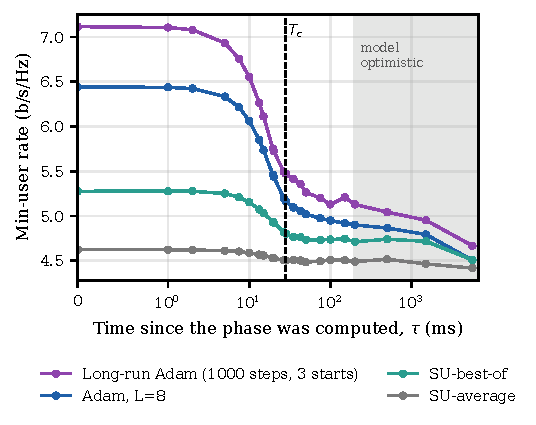
\includegraphics[width=0.92\columnwidth]{figures/fig_aging.pdf}
\caption{Kullanıcılar 1.5~m/s hızla yürürken, ön kodlayıcı tazelenerek, $t=0$ anında sabitlenen bir fazın en düşük kullanıcı hızı. Kesikli: $T_c=28.2$~ms. Gölgeli: 200~ms'nin ötesinde model iyimserdir.}
\label{fig:aging}
\end{figure}

\subsection{Birkaç Adımdan Sonra Ek Yinelemeler Yararlı Olmaktan Çıkar}
\label{sec:res_optimum}
Şekil~\ref{fig:optimum}, Adam adım sayısını SU-average'dan (4.624~b/s/Hz) başlayarak tarar. $t=0$ hızı her adımda artar: $L=1$'de 5.412'den $L=48$'de 7.037~b/s/Hz'e. Etkin hız ise artmaz: $L=4$--$6$'da tepe yapar (6.7--10.0~ms'de 5.980, 5.982 ve 5.970~b/s/Hz) ve diğer her adım sayısı anlamlı ölçüde daha düşüktür. $L=48$'de, oradaki $t=0$ hızı \%13.2 daha yüksek olmasına rağmen, etkin hız tepenin \%14.0 (\%95 GA \%12.5--15.5) altındadır. \eqref{eq:marginal} ifadesi açısından, $L=4$'ten $6$'ya geçmek $t=0$ anında 0.188~b/s/Hz ekler ama eskimede 0.198'e mal olur.

Optimum, Adam'ın ya da adım boyunun yapay bir sonucu değildir. 0.25, 0.75 ve 1.0 adım boyları optimumu $L=6$, $4$ ve $5$'e yerleştirir; $L=48$'deki kayıplar \%11.5, \%13.7 ve \%11.3'tür. Armijo en dik çıkışı $L=4$'te tepe yapar (6.015~b/s/Hz). İlk adımlarda Adam'dan daha fazla kazanır ancak adım başına maliyeti Adam'ınkinin 1.26 katıdır ve iki tepe istatistiksel olarak berabedir (fark 0.033, GA $-0.001$ ile 0.064 arası). Armijo'nun adım başına maliyeti Adam'ınkinin 1.0, 1.2, 1.4, 1.6 ve 2.0 katı olduğunda, en iyi etkin hızı Adam'ınkine göre $+0.147$, $+0.050$, $-0.013$, $-0.079$ ve $-0.197$~b/s/Hz olur: iki klasik optimize edici arasında bile sıralamayı gecikme belirler.

\begin{figure}[t]
\centering
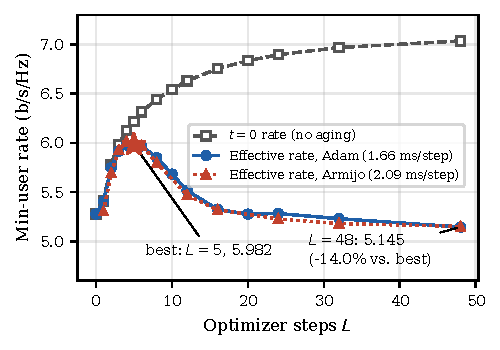
\includegraphics[width=0.92\columnwidth]{figures/fig_intrinsic_optimum.pdf}
\caption{Adım taraması (eskime kümesi). $t=0$ hızı $L$ ile artar; etkin hız $L=4$--$6$'da tepe yapar ve $L=48$'de \%14.0 daha düşüktür. Armijo (adım başına 2.09~ms) aynı biçimi gösterir. $L=0$: 0.05~ms'de SU-best-of (5.276; ölçülen 2.5~ms'sinde 5.272).}
\label{fig:optimum}
\end{figure}

\subsection{Optimumu Tek Bir Sayı Belirler}
\label{sec:res_scaling}
Optimize edilmiş bir gerçekleme adım başına daha hızlı olurdu. Bu nedenle Şekil~\ref{fig:scaling}, Adam'ın adım süresini ölçülen değerin 0.01 ila 3 katı arasında ölçekler, yani $x$'i $2.5\times10^{-4}$'ten $7.5\times10^{-2}$'ye kadar; bu kurulum $x=2.5\times10^{-2}$ noktasındadır ve aynı eksen buradakinden 100 kata kadar daha yavaş ya da 3 kat daha hızlı kullanıcıları da kapsar. En iyi adım sayısı düzenli olarak azalır: en küçük $x$'te 96 adım, ardından 48, 24--32, 12--16, burada 4--6 ve en büyükte 2. En küçük $x$'te yakınsama neredeyse bedavadır ($L=256$'ya kadar koşmanın maliyeti \%1.5, GA \%1.3--1.8); yakınsamanın maliyeti $x\approx 2.5\times10^{-3}$ civarında yaklaşık \%21 ile tepe yapar. $x\ge 2.5\times10^{-2}$ için $L=256$ 200~ms ufkunun ötesindedir; dolayısıyla maliyeti, olsa olsa, olduğundan düşük gösterilmektedir. Bu nedenle yakınsamanın zarar verip vermediği, genel olarak RIS optimizasyonunun değil, rejimin bir özelliğidir. GPU ya da NPU gibi daha hızlı donanım adımı kısaltır ve böylece optimumu kaydırır, ancak onu ortadan kaldırmaz: modelde (Önerme~1) her $x>0$ için bir iç optimum vardır ve ölçümlerde optimum yüz kat daha hızlı bir adıma kadar varlığını sürdürür; orada 96 adımdadır.

Önerme~1'in dayandığı iki yasa da yaklaşık olarak geçerlidir. Eskime kaybı karesele yakındır (her $L$ için $R^2\ge 0.98$, $\tau\le 10$~ms için uydurulmuş) ve $\kappa_L$, $L=1$'de 7.8'den $L=48$'de 25.1'e büyür. Yakınsama açığı kabaca bir kuvvet yasasını izler; $\gamma=0.93$ olmakla birlikte uydurma aralığına bağlı olarak 0.56 ile 1.19 arasında değişir, dolayısıyla öngörülen üs $-0.78$ ile $-0.63$ arasındadır. $L^\star(x)$'in ölçülen eğimi $-0.675$'tir (\%95 GA $-0.692$ ile $-0.655$ arası) ve bu aralığın içindedir; dolayısıyla model üssü ancak yaklaşık $\pm 0.08$ hassasiyetle belirler. Kapalı biçim~\eqref{eq:Lstar}, her $x$'te ölçülen optimumun 1.27 çarpanı içindedir (burada 5.3'e karşı 5). Bu bir örneklem içi denetimdir: $\kappa_L$, optimumların ortaya çıktığı gecikmeler (1.6--10~ms) üzerinde uydurulmuştur. Önerme~1'in dengesi nicel olarak geçerli değildir (oran 0.19 ile 1.65 arasında değişir); dolayısıyla model optimumun nerede bulunduğunu ve neden kaydığını açıklar, iki kaybın nasıl bölüştüğünü değil.

Daha büyük bir $8\times 8$ yüzey ($N=64$) yakınsanmış hızı yükseltir (8.48'e karşı 7.10~b/s/Hz) ancak her adım süresi çarpanında aynı en iyi adım sayısına sahiptir; bu, optimumu doğrular, ama üssü bağımsız olarak doğrulamaz. Adımı bizim kodumuzda yalnızca 1.04 kat daha pahalı olduğundan neredeyse aynı $x$'te yer alır; maliyeti $N$ ile büyüyen bir gerçekleme onu daha az adıma kaydırırdı.

\begin{figure}[t]
\centering
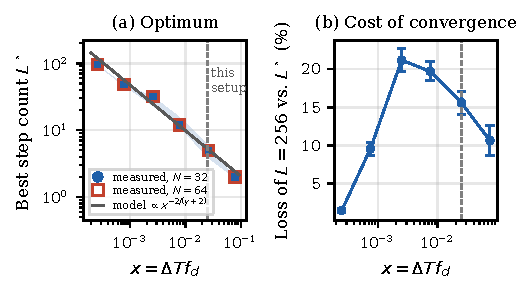
\includegraphics[width=\columnwidth]{figures/fig_step_scaling.pdf}
\caption{Adım süresi ölçülen değerin 0.01 ila 3 katı arasında ölçeklenmiş Adam. (a)~$N=32$ (gölgeli: en iyiden anlamlı ölçüde düşük olmayanlar) ve $N=64$ için en iyi adım sayısı; çizgi: kapalı biçim~\eqref{eq:Lstar}. (b)~$L^\star$ yerine $L=256$'ya kadar koşmanın kaybı ($N=32$), \%95 eşli GA'larla. Kesikli: bu kurulum.}
\label{fig:scaling}
\end{figure}

\subsection{Standartlaştırılmış Hızlar ve Kanal Edinme Gecikmesi}
\label{sec:res_sensitivity}
Tablo~\ref{tab:speeds}, ana ölçümleri aynı senaryolarda, 40~ms'ye kadar 0.5~ms aralıklı bir zaman ızgarasında, standartlardaki kullanıcı hızlarında ve bunlardan daha yüksek iki hızda tekrarlar: 3GPP iç mekân sıcak nokta değerlendirmesinde kullanılan 3~km/h~\cite{3gpp_tr38913}; iç mekân hareketliliğinin değerlendirildiği IMT-2020 yaya sınıfının üst ucu olan 10~km/h~\cite{itu_m2410}; ve yaya sınıfının ötesinde, 18~km/h (5~m/s, araç sınıfında bizim seçimimiz) ile yoğun kentsel değerlendirmenin 30~km/h'i~\cite{3gpp_tr38913,itu_m2410}. Kanal edinme gecikmesi olmadan iki bulgu da---bir optimal adım sayısının varlığı ve yavaş çözücülerin kaybetmesi---her hızda geçerlidir. Optimum 3~km/h'te 8 adımdan 10~km/h'te 3'e, 18~km/h'te 2'ye ve 30~km/h'te 1'e kayar. $L=48$'e kadar koşmanın maliyeti 3~km/h'te \%14.5 (\%95 GA \%13.1--16.1), 10~km/h'te \%10.5'tir (\%9.0--11.9). SU-best-of her hızda koordinat inişinin 0.25--0.42~b/s/Hz, uzun koşulu Adam'ın 0.45--0.69 önündedir ve eşli GA'lar sıfırın üzerindedir (yavaş çözücüler için iyimser değerler). 18 ve 30~km/h'te $L=48$ güvenilir ufkun (60 ve 36~ms) ötesindedir; dolayısıyla bu maliyet yaklaşıktır. 3.43~ms kanal edinme gecikmesiyle optimum 18 ve 30~km/h'te çözümlenemez ve 30~km/h'te SU-best-of ile koordinat inişi artık anlamlı ölçüde farklı değildir. Bu daha ince ızgarada, 1.5~m/s'de $L=4$--$6$ birbirinin \%0.5'i içindedir ve $L=48$'e kadar koşmanın maliyeti \%14.2'dir (ana taramada \%14.0).

\begin{table}[t]
\centering
\caption{Standartlaştırılmış ve daha yüksek kullanıcı hızları (eskime kümesi, kanal edinme gecikmesi yok): eş evrelilik süresi, normalize adım maliyeti, en iyi adım sayısı (\%0.5 içindeki aralık), Adam'ı $L=48$'e kadar koşmanın maliyeti ve $\Delta$: etkin hızda SU-best-of eksi koordinat inişi (b/s/Hz). 0.5~ms'lik bir ızgarada hesaplanmıştır; bu nedenle değerler Tablo~\ref{tab:aging} ve Şekil~\ref{fig:optimum} değerlerinden biraz farklı olabilir. $^\dagger$Güvenilir ufkun ötesinde; yaklaşık.}
\label{tab:speeds}
\footnotesize
\setlength{\tabcolsep}{3pt}
\begin{tabular}{rlrrlrr}
\toprule
km/h & Kaynak & $T_c$ (ms) & $x$ & $L^\star$ & $L{=}48$ & $\Delta$ \\
\midrule
3 & 3GPP~\cite{3gpp_tr38913} & 50.8 & 0.014 & 8 (6--8) & 14.5\% & $+0.27$ \\
5.4 & bu çalışma & 28.2 & 0.025 & 4 (4--6) & 14.2\% & $+0.31$ \\
10 & ITU~\cite{itu_m2410} & 15.2 & 0.046 & 3 & 10.5\% & $+0.25$ \\
18 & bu çalışma, ITU araç & 8.5 & 0.083 & 2 & 8.0\%$^\dagger$ & $+0.42$ \\
30 & ITU, kentsel & 5.1 & 0.139 & 1 & 4.3\%$^\dagger$ & $+0.42$ \\
\bottomrule
\end{tabular}

\end{table}

Konuşlandırılmış bir sistem, optimize etmeden önce pilotlara ve geri beslemeye de zaman harcar. Ana ızgarada, 1--3~m/s'de 0--10~ms'lik bir kanal edinme gecikmesi eklemek optimumu \eqref{eq:marginal} ifadesinin öngördüğü biçimde kaydırır (1.5~m/s'de $L=4$--$6$'dan $L=3$--$4$'e); $T_c/2$'nin üzerindeki gecikmeler dışarıda bırakıldığında (yalnızca 10~ms ile 3~m/s), $L=48$'e kadar koşmanın maliyeti \%2.9--14.7'dir. Optimum yanlış bir hız varsayımını da tolere eder: kullanıcılar 1.8~m/s ile hareket ederken $L$'yi 1.5~m/s için seçmenin maliyeti \%0.5'ten azdır ve ızgaramızdaki hiçbir varsayılan ve gerçek hız çifti \%5.7'den fazlasına mal olmaz.

\emph{Paylaşılan saçılma kazançları.} Fiziksel bir kanalda olduğu gibi tüm BS antenleri için saçıcı başına tek bir kazanç kullanıldığında mutlak hızlar düşer (Tablo~\ref{tab:speeds} ızgarasında 1.5~m/s'de Adam'ın en iyi etkin hızı: 5.984 yerine 5.398~b/s/Hz), ancak bulgular geçerliliğini korur: $L^\star$ 1.5~m/s'de 4--6'da ve 10~km/h'te 3'te kalır, $L=48$'e kadar koşmanın maliyeti sırasıyla \%17.7 (GA \%15.8--19.5) ve \%14.2'dir ve SU-best-of koordinat inişinin ve uzun koşulu Adam'ın önünde kalır (eşli GA'lar sıfırın üzerinde).

\subsection{Periyodik Çalışma: Periyodu Pilotlar Belirler, Kısa Güncellemeler Yeterlidir}
\label{sec:res_tracking}
Tablo~\ref{tab:tracking}, Tanım~3'teki denetleyicinin benzetimini yapar. Ne sıklıkla güncelleme yapılacağına pilot ek yükü karar verir. Bedava pilotlarla, sıcak başlangıçlı iki adımla yapılan art arda güncellemeler en iyisidir (6.36~b/s/Hz); 0.86~ms pilotla en iyi periyot 10--20~ms'dir; 3.43~ms ile, her 80~ms'de bir yapılan güncellemeler (sıcak başlangıç) ve 48 adımlı art arda güncellemeler (soğuk başlangıç) istatistiksel olarak berabedir. Değişmeyen şey, kısa güncellemelerin yeterli olmasıdır: her satırda, en fazla 8 adımlı ve en iyiden anlamlı ölçüde düşük olmayan bir politika vardır. Sıcak başlangıç, pilotlar kısa olduğunda 0.53~b/s/Hz'e kadar kazanç sağlar, 3.43~ms pilotlarla ise anlamlı hiçbir kazanç sağlamaz.

\begin{table}[t]
\centering
\caption{Periyodik yeniden optimizasyon (eskime kümesi): $T_{\mathrm{p}}$ pilot süreleri için en iyi güncelleme periyodu $U$ (ms; b2b = art arda) ve güncelleme başına adım $L$, zaman ortalamalı etkin hızla (b/s/Hz) birlikte. Sıcak$-$soğuk: en iyi iki politikanın eşli farkı; $^\S$anlamlı değil.}
\label{tab:tracking}
\footnotesize
\setlength{\tabcolsep}{5.5pt}
\begin{tabular}{r|rrr|rrr|r}
\toprule
 & \multicolumn{3}{c|}{Soğuk başlangıç} & \multicolumn{3}{c|}{Sıcak başlangıç} & \\
$T_{\mathrm{p}}$ (ms) & $U$ & $L$ & hız & $U$ & $L$ & hız & sıcak$-$soğuk \\
\midrule
0 & b2b & 3 & 5.83 & b2b & 2 & 6.36 & +0.53 \\
0.86 & 20 & 3 & 5.24 & 10 & 3 & 5.51 & +0.28 \\
1.71 & b2b & 48 & 5.08 & 20 & 3 & 5.17 & +0.09 \\
3.43 & b2b & 48 & 4.98 & 80 & 24 & 4.99 & +0.01$^\S$ \\
\bottomrule
\end{tabular}

\end{table}

\subsection{Öğrenilen Bir Güncelleme Kuralı Adım Başına Kazanır ama Milisaniye Başına Kaybeder}
\label{sec:res_reversal}
Bu karşılaştırma, hesaplama verimliliğini yalıtmak için statik kümeyi ve $t=0$ hızlarını kullanır. Eşit adım sayısında öğrenilen kural, her $L\in\{1,2,4,8,16\}$ bütçesinde ayarlanmış Adam'ı yener (Şekil~\ref{fig:eqms}(a)) ve test senaryolarının \%68--84'ünde kazanır. Ancak tek bir öğrenilen adım, 2.7--4.0 Adam adımı kadar zaman alır. Ölçülen zaman ekseninde (Şekil~\ref{fig:eqms}(b)), beş zamanlama turunun her birinde, her öğrenilen yapılandırma hem daha hızlı hem daha iyi olan bir Adam yapılandırması tarafından baskınlanır. Örneğin $L=4$ ile öğrenilen kural 5.285~b/s/Hz için 18.41~ms gerektirirken $L=8$ ile Adam 5.380~b/s/Hz için 13.48~ms gerektirir. Eşit adım sıralaması tamamen tersine döner. Eskime burada dahil edilmemiştir; her çiftte daha yavaş olan öğrenilen yapılandırma olduğundan, eskimenin aradaki farkı açması beklenirdi. Ancak maliyet oranı, bu gerçeklemenin tek bir CPU iş parçacığı üzerindeki bir özelliğidir: ağın matris çarpımlarını Adam'ın adımından daha fazla hızlandıran donanımda bu tersine dönme zayıflayabilir.

\begin{figure*}[t]
\centering
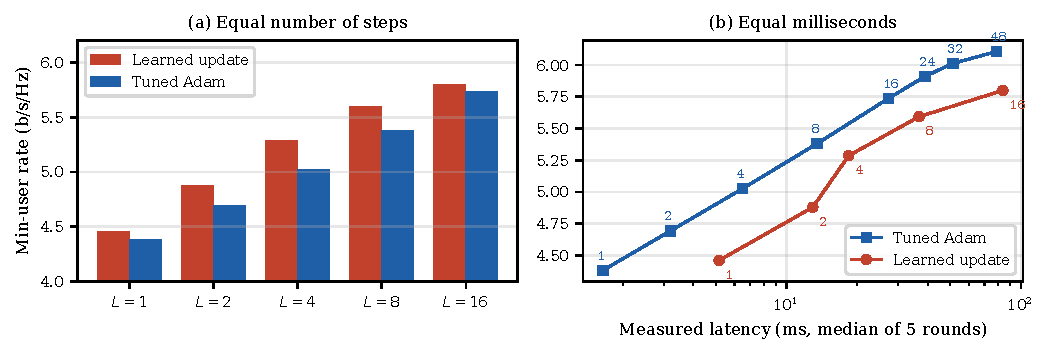
\includegraphics[width=\textwidth]{figures/fig_equal_step_vs_ms.pdf}
\caption{Öğrenilen güncelleme kuralı ile ayarlanmış Adam'ın karşılaştırması (statik test kümesi, 600 senaryo, $t=0$ hızları, tek CPU iş parçacığı). (a)~Eşit adımda öğrenilen kural her bütçede öndedir. (b)~Ölçülen gecikme ekseninde (etiketler: adım sayısı $L$), her öğrenilen yapılandırma Adam eğrisinin altında ve sağında yer alır: baskınlanmıştır.}
\label{fig:eqms}
\end{figure*}

\subsection{Taze Hüzme Varsayımı Önemlidir}
\label{sec:res_beam}
Ana sonuçlar, yalnızca RIS fazı eskirken BS'nin ön kodlayıcısını güncel kanaldan tazelediğini varsayar. Hüzme kümesinde, bunun yerine ön kodlayıcıyı $t=0$ anındaki hâliyle tutmak hızın onlarca milisaniye içinde çökmesine yol açar: $T_c$ anında hız, her faz seçimi için, taze hüzmeye göre 11.7--14.2$\times$ daha düşüktür ve Adam'ın ($L=8$) fazıyla yalnızca 5~ms yaşındaki bir ön kodlayıcı bile hızı 5.228'den 1.736~b/s/Hz'e düşürür (hüzme kümesi hızları Tablo~\ref{tab:aging} ile karşılaştırılabilir değildir). Ön kodlayıcıyı tazelemek ucuzdur (0.12~ms, bir Adam adımından yaklaşık 13 kat kısa), ancak birkaç milisaniyede bir etkin kanal pilotları gerektirir; bunların yayın süresi Bölüm~\ref{sec:res_robust} kapsamında hesaba katılır.

\subsection{Pilotlara, Kestirim Hatasına ve Faz Çözünürlüğüne Dayanıklılık}
\label{sec:res_robust}
Bu denetimler eskime kümesini ve Bölüm~\ref{sec:method} kapsamında yeniden ölçülen gecikmeleri (Adam adımı başına 1.33~ms) kullanır. Yapılandırmalar bağımsız bir hareketlilik çekilişinde (tohum 12) seçilir ve eşli GA'larla raporlanır; $L^\star$ eskime kümesinde okunur.

\emph{Ön kodlayıcı pilotları.} Ön kodlayıcı, veri taşımayan dört pilot sembolünden her $T_{\mathrm{r}}$~ms'de bir tazelendiğinde ($T_{\mathrm{r}}$ yönteme göre seçilir) ve en düşük kullanıcı hızı, pilotlar düşülerek, konuşlandırmadan sonraki $W$~ms boyunca ortalandığında ($\bar{R}_W$), seçilen yapılandırma bedava tazelemeyle 5.21~b/s/Hz'e, 15, 30 ve 60~kHz alt taşıyıcı aralığında ise 3.54, 4.00 ve 4.33~b/s/Hz'e ulaşır ($W=50$~ms, $T_{\mathrm{r}}=1$--2~ms). Bu yapılandırma 6--8 Adam adımı kullanır; 3--20 adım onunla berabedir ve koordinat inişi ile uzun koşulu Adam anlamlı ölçüde geridedir. $W=25$, 50 ve 100~ms için seçilen adım sayıları 5, 6--8 ve 16--20'dir (bedava tazelemeyle 16--24); 100~ms'de, pilotlarla, altı adım 0.02--0.04~b/s/Hz aşağıda kalır. Ancak SU-best-of'a karşı, koordinat inişi (0.70~s sonra, güvenilir ufkun ötesinde, modelin onu kayırdığı bölgede konuşlandırılır) pilotlarla $W=50$~ms'de berabere kalır ve bedava tazelemeyle ya da $W=100$~ms'de 0.09--0.18~b/s/Hz önde olur (15~kHz hariç); onu her pencerede yalnızca ayarlanmış Adam yener.

\emph{Kusurlu kanal bilgisi.} Ortalama kanal gücüne göre $1/(1+\rho)$ güçte kestirim hatasıyla ($\rho$: pilot sinyal-gürültü oranı; 30~dB'de RIS--kullanıcı kanalı için senaryo başına medyan 22.6~dB), faz $t=0$ kestiriminden ve ön kodlayıcı taze bir kestirimden alındığında, en iyi etkin hız 30 ve 20~dB'de 6.08'den 3.54 ve 1.40~b/s/Hz'e düşer (ikincisi, tek başına doğrudan bağlantının değeri olan 1.74'ün altındadır); 10~dB ve altında hızlar sıfıra yakındır ve Adam ile SU-best-of berabedir. Pilotlar da hesaba katıldığında ($\bar{R}_{50}$), Adam 30~dB'de SU-best-of'un 0.05--0.06~b/s/Hz önündedir ve 20~dB'de onunla berabedir; koordinat inişi ve uzun koşulu Adam anlamlı ölçüde geride kalmaya devam eder.

\emph{Ayrık fazlar.} Adam'ın (adım boyu 0.5) ve SU-best-of'un fazlarını hiçbir zaman maliyeti olmadan $2^b$ düzeye yuvarlamak içsel bir optimumu korur ($b=1$, 2, 3 için $L^\star=5$, 6, 6; $L=48$'in maliyeti \%9.5, \%14.1, \%14.9). $2^b$ düzey üzerinde ayrık koordinat inişi (16--501~ms), $b=3$'te ve iki ya da daha fazla taramayla $b=2$'de yuvarlanmış SU-best-of'un anlamlı ölçüde gerisindedir. $b=1$'de tek bir taramayla (16~ms) seçilir: yuvarlanmış SU-best-of'un 0.25~b/s/Hz (GA 0.16--0.33) üzerindedir ve en iyi yuvarlanmış Adam ile berabedir ($-0.04$, GA $-0.11$ ile 0.02 arası).

\section{Sonuç}
\label{sec:conclusion}

Kullanıcılar hareket ederken bir baz istasyonunun hangi RIS faz optimize edicisini ve ne kadar süreyle koşturması gerektiğini sorduk. Her yöntemin ihtiyaç duyduğu süreyi hesaba katarak şu bulgulara ulaşıyoruz.
\begin{enumerate}
    \item \textbf{Hız, hassasiyeti yener.} Ölçülen adım maliyetlerinde yavaş çözücüler, koordinat taramalarının sayısı ayarlanmış olsa bile, milisaniyeler süren tek kullanıcılı bir sezgisel yönteme yenilir; kanal edinme gecikmesi olmadığında bu, 3 ile 30~km/h arasındaki her hızda geçerlidir (yavaş çözücüler için iyimser değerlerle). Daha uzun pencereler üzerinden ortalandığında koordinat inişi sezgisel yöntemle berabere kalabilir ya da onu geçebilir, ancak ayarlanmış Adam'ın gerisinde kalır.
    \item \textbf{Birkaç adım optimaldir.} Faz birkaç on milisaniyede bir yenilendiğinde Adam'ın dar bant etkin hızı bir avuç adımdan sonra tepe yapar ve ardından düşer (fazı daha uzun tutmak, düz bir optimumu yukarı kaydırır); optimum, 3~km/h hızda 8 adımdan, IMT-2020 yaya sınıfının üst ucu olan 10~km/h hızda 3 adıma kayar.
    \item \textbf{Optimumu tek bir sayı belirler.} En iyi adım sayısını Doppler frekansına göreli adım süresi, $x=\Delta T f_d$, belirler ve bu sayı yaklaşık olarak $x^{-2/(\gamma+2)}$ gibi ölçeklenir (ölçülen üs $-0.675$); yüz kat daha hızlı bir gerçekleştirmeyle yakınsama neredeyse bedava hale gelir.
    \item \textbf{Güncelleme periyodunu pilotlar belirler.} Sürekli işletimde ne sıklıkla güncelleme yapılacağına pilot ek yükü karar verir; kısa güncellemeler (en fazla 8 adım) yeterlidir.
    \item \textbf{Öğrenme saat karşısında kazanmalıdır.} Eşit adımlarda kazanmak yeterli değildir: öğrenilen güncelleme kuralı (statik küme, tek CPU iş parçacığı), her adıma ölçülen süresi maliyet olarak yansıtıldığı anda baskınlanmış olur.
\end{enumerate}
Burada nicelendirilen rejimde gecikme, hareketli RIS için ikincil bir ölçüt değildir: hangi yöntemin en iyi olduğuna o karar verir.

\emph{Pratik kurallar.} Adım sayısını yakınsamaya göre değil; $x$ değerine, kanal edinme gecikmesine ve fazın ne kadar süre tutulacağına göre seçin. Güncelleme periyodunu pilot ek yüküne göre seçin. Yöntemleri, her bütçede ayarlanmış bir klasik taban çizgisine karşı ölçülmüş gecikme üzerinden karşılaştırın ve eşit adımdaki kazanımlar yerine baskınlığı raporlayın.

\emph{Sınırlılıklar.} Ana sonuçlar, BS'nin ön kodlayıcısını güncel kanaldan kusursuz bilgiyle yeniden hesapladığını varsayar. Pilot yayın süresi (\%17--32 daha düşük hızlar), kestirim hatası ve 2--3 bitlik fazlar yavaş çözücüleri ayarlanmış Adam'ın gerisinde bırakır; tek bitte tek taramalı bir arama en iyi yuvarlanmış Adam ile berabere kalır ve 10~dB ve altındaki pilot sinyal-gürültü oranlarında hızlı yöntemler birbirinden ayırt edilemez (Bölüm~\ref{sec:res_robust}). RIS anahtarlama süresi (\cite{Zhao2024OJCOMS} çalışmasında $\ge$0.72~ms) modellenmemiştir ve tek bir geometri vardır. Gecikmeler tek iş parçacıklı Python'dan gelmektedir: yalnızca koordinat inişi derlenirse (62--63 kat daha hızlı) Python Adam'ı geçer, ancak tüm yöntemlerin eşit ölçüde hızlandırılması ayarlanmış Adam'ı önde tutar; normalize adım maliyeti sonuçları başka hızlara ve, yaklaşık olarak, başka taşıyıcılara taşır. Yarı tanımlı gevşetme~\cite{Wu2019TWC}, WMMSE~\cite{Choi2024TCOM} ve manifold yöntemleri zamanlanmamıştır; uzun koşulu Adam ise yalnızca sabit bir bütçede zamanlanmıştır. İlk bir OFDM kontrolünde iç optimum, 20~MHz'de merkez frekans optimizasyonu için geçerliliğini korumuştur; ancak 50--100~MHz'de 48 adım, 16 yapılandırmadan yalnızca 3 tanesinde anlamlı ölçüde daha kötü olmuştur.


\section*{Teşekkür}
\emph{Yapay zekâ araçlarının kullanımı.} IEEE politikası uyarınca, bu makalenin hazırlanmasında yapay zekâ asistanı Claude'un (Anthropic) kullanıldığını beyan ederiz: bütün bölümlerin metnini taslak hâline getirmek ve düzenlemek, yazarların benzetim altyapısını Python'a aktarmak, deneyleri tanımlayan ve sonuçları denetleyen yazarlarla birlikte deney ve analiz betiklerini geliştirmek, kayıtlı sonuçlardan şekil ve tabloları üretmek ve kaynakları kontrol etmek için. Çalışmayı yazarlar tasarlamış, bütün analizleri yönlendirmiş, her sonucu ve kaynağı doğrulamıştır ve içeriğin bütün sorumluluğunu taşır.

\section*{Veri ve Kodun Erişilebilirliği}
Her tablo ve şekli üreten betikler ve bunların okuduğu kayıtlı ölçüm dosyaları \url{https://github.com/sedasavascisen/ris-latency-mobility} adresinde erişilebilirdir.

\bibliographystyle{IEEEtran}
\bibliography{../makale2_revizyon/references/references}

\end{document}
